%%%%%%%%%%%%%%%%%%%%%%%%%%%%%%%%%%%%%%%%%%%%%%%%%%%%%%%%%%%%%%%%%%%%%%%%%%%
%
% Plantilla para un artículo en LaTeX en español.
%
%%%%%%%%%%%%%%%%%%%%%%%%%%%%%%%%%%%%%%%%%%%%%%%%%%%%%%%%%%%%%%%%%%%%%%%%%%%

% Qué tipo de documento estamos por comenzar:
\documentclass[a4paper]{article}
% Esto es para que el LaTeX sepa que el texto está en español:
\usepackage[spanish]{babel}
\selectlanguage{spanish}
% Esto es para poder escribir acentos directamente:
\usepackage[utf8]{inputenc}
\usepackage[T1]{fontenc}



%% Asigna un tamaño a la hoja y los márgenes
\usepackage[a4paper,top=3cm,bottom=2cm,left=3cm,right=3cm,marginparwidth=1.75cm]{geometry}

%% Paquetes de la AMS
\usepackage{amsmath, amsthm, amsfonts}
%% Para añadir archivos con extensión pdf, jpg, png or tif
\usepackage{graphicx}
\usepackage[colorinlistoftodos]{todonotes}
\usepackage[colorlinks=true, allcolors=blue]{hyperref}

%% Primero escribimos el título
\title{Universidad 4.0}
\author{Armijo, Daniela\\
  \small daniarmijo@icloud.com
  \and
  Calvo, Nicolás\\
  \small ricardocalvo1997@gmail.com
  \and
  Kudaka, Matias\\
  \small matiaskudaka@gmail.com
  \and
  Olmedo, Matías\\
  \small olmedomn@live.com.ar
  \and
  Orozco, Marianela\\
  \small orozcomarianela10@gmail.com\\
  \small Universidad Tecnológica Nacional\\
  \small San Rafael - Mendoza
  \and
  Ramirez, Beatriz\\
  \small beatriz.vgb@gmail.com\\
  \date{}
}

%% Después del "preámbulo", podemos empezar el documento

\begin{document}
%% Hay que decirle que incluya el título en el documento
\maketitle

%% Aquí podemos añadir un resumen del trabajo (o del artículo en su caso) 
\maketitle
\begin{abstract}
Los problemas que se encuentran durante el proceso de inscripción y cursado en la FRSR, pueden resolverse aprovechando los avances tecnológicos.
\end{abstract}

%% Iniciamos "secciones" que servirán como subtítulos

\section{Planteamiento del problema}

Hoy en día la administración pública nos permite acceder a una gran variedad de trámites en línea, como gestionar la renovación del DNI, el certificado de antecedentes personales y mucho más, simplemente haciendo uso de distintas aplicaciones. Todo esto lo podemos hacer desde nuestro dispositivo móvil o computadora, para ello necesitamos de los sistemas informáticos, las aplicaciones móviles, las redes informáticas y muy especialmente la seguridad. Pero aún así, existen aún muchos trámites que se deben hacer en forma personal, y para los cuales nos piden certificados o formularios que debemos imprimir o fotocopiar, o más aún, retirarlos de alguna oficina o registro, con el pago de algún sellado. Por ejemplo, para muchos trámites nos solicitan la partida nacimiento, legalizada con una antigüedad no mayor a 3 meses. Burocracia, papeleo, firmas en papel, esto no sería necesario si contásemos con un sistema único donde estén todos nuestros datos almacenados, de donde podamos obtenerlos y transmitirlos de una institución a otra sin necesidad de oficinas intermediarias ni de realizar pagos. También el uso de sistemas informáticos diferentes no permite optimizar este recurso. 

Llevando esto al plano de nuestra facultad regional San Rafael de la UTN, vemos que sucede algo similar. En nuestra institución, los problemas con la Tecnicatura Universitaria en Programación se han generado porque falta un sistema que controle el volumen de información que generan/solicitan más de 500 personas. Teniendo en cuenta que hay una tendencia al crecimiento de la demanda de carreras/cursos con modalidad virtual o blended-learning, estos problemas van a ir en aumento. Enumeremos algunos de ellos.

El proceso de inscripción es lento, se solicitan fotocopias de DNI, títulos, rellenar formularios y llevarlos en persona a la institución. Ya existe un sistema (miArgentina) que tiene los datos personales, DNI digital, etc. que se utilizan en este proceso. El sistema de la Universidad debería estar conectado de alguna manera a este para recibir la información necesaria. Lo mismo debería pasar con el título secundario, la DGE tiene un sistema que es el GEM en el cual está toda la trayectoria escolar de los estudiantes.  El sistema de inscripción a la facultad debería recurrir a estos para tomar esos datos, sin necesidad de recurrir al papel, viajes hasta el lugar, lugar físico para guardar legajos, personas para gestionar. Son gastos que podrían reducirse o eliminarse. Incluso contar con un sistema de toma de medidas biométricas, para reconocimiento facial, y de toma de firmas electrónicas legales. Está claro que el lugar físico debería reemplazarse por “nubes” para guardar los datos que son “espacios virtuales” que, aunque también generan gastos, son menores, considerando también el mantenimiento y luego el peligro y riesgos que implica mantener en una institución volúmenes importantes de legajos en papel. Ha pasado que en instituciones se han perdido por incendios e inundaciones. Obviamente que el resguardo de datos en la nube también implica el uso de seguridad informática, pero es menos propenso a riesgos y a pérdidas, filtrado, etc. 

El problema que acarrea estos trámites continúa al momento de rendir un examen final. Inscripciones se hacen por sistema, pero el sistema es susceptible de errores. Los estudiantes se quejan del mismo, no es claro, se inscriben y no aparecen, etc. Luego los profesores no tienen un sistema para asentar las notas, las notas se pasan por escrito en una planilla, por cada especialidad va una planilla por duplicado, la misma luego tienen que firmarla los docentes y luego se vuelca al sistema. Esto genera atrasos, errores y hasta pérdidas de información. Además de que se presta a manejos indeseables.  

El sistema académico que así se llama, aunque tiene la capacidad para registrar varios datos, no se usa en su totalidad. Ejemplo: los profesores deben llevar cada uno por su parte un listado de alumnos, con la información que los alumnos quieran dar, para tomar asistencia, colocar notas. Lo ideal sería contar son un sistema que permita a cada profesor acceder a la trayectoria de cada alumno, colocar sus asistencias y notas. Un sistema que sea igual para todas las cátedras, automático, calculando porcentajes de asistencia, promedios, y que le asigne automáticamente a cada alumno su estado (libre, regular, aprobado)
Esto implicaría como dijimos, un ahorro significativo en: espacio físico, personal, artículos de librería y oficina, etc. A la vez que la eficiencia del sistema sería mayor. 

La cuestión se extiende también a la extensión de título. Por sistema, ya el alumno no tendría que esperar tiempo para recibir su título, automáticamente, rinde su última materia y se asienta en sistema, el título digital está a su disposición, con la misma validez que el cartón (el cartón ya no sería necesario, lo cual ahorraría también bastante dinero, además del tiempo). Esto exige, como en cada etapa de este sistema, la completa seguridad del mismo. 


\section{La propuesta}

La idea es unificar todas estas tareas administrativas que el estudiante debe hacer en un único sistema, para luego hacerlo extensivo a todas las instituciones, de manera tal de lograr la conexión entre ellas, y evitar presentación de papeles, fotocopias, rellenado de formularios, sellados, pagos, duplicación de información, etc. Los objetivos son:
-	Reducir el número de empleados que realizan estas tareas manualmente
-	Desarrollar procesos (contables, de inscripciónes, de certificaciones, etc) sin papel.
-	Hacer que los datos de gestión, personales, etc. Estén centralizados y disponibles a nivel de cualquier institución que los necesite, con un nivel de seguridad máximo. Los datos personales sólo podrán ser accesibles para una institución, mediante al menos la doble autenticación de la persona en cuestión. 
Un ejemplo a nivel mundial ha sido desarrollado con éxito en Estonia; lo llaman proyecto de centralización de los servicios compartidos estatales. “En el punto de partida había 253 agencias estatales con contabilidad financiera independiente, contabilidad de recursos humanos y sistemas de cálculo de nómina. Había 14 soluciones de software de contabilidad diferentes y 11 soluciones de software de contabilidad de recursos humanos diferentes en uso y no había un sistema de informes común. Los sistemas informáticos de función principal no estaban vinculados a software de contabilidad financiera o de personal. Todas las agencias gastaron dinero por separado en el desarrollo de esos diferentes softwares.”
Como resultado de la aplicación del proyecto de sistematización y unificación de los sistemas informático, se ha reducido el número de empleados, se ha centralizado la información, los empleados estatales están satisfechos porque se ha reducido la burocracia lo que ha hecho que los procesos sean mucho más rápidos. También se ha logrado una importante reducción de la corrupción en el estado. Para visualizar la diferencia entre ambos países, usamos el Indice de Percepción de la Corrupción, publicados por Transparecy Internacional, como puede verse en la fig. \ref{fig:Imagen1}.

\begin{figure}
\centering
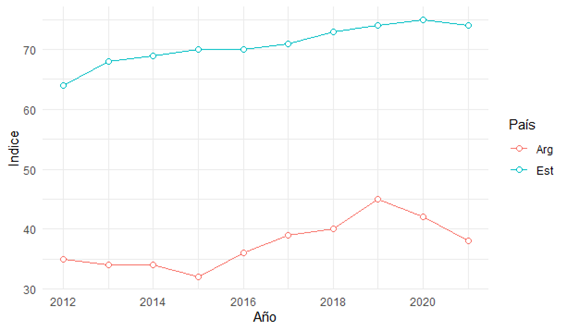
\includegraphics[width=0.5\textwidth]{Imagen1.png}
\caption{\label{fig:Imagen1}Indice de Percepción de la Corrupción.}
\end{figure}

“El Índice de Percepción de la Corrupción clasifica 180 países y territorios según el nivel de percepción de la corrupción en el sector público de cada uno, en una escala de cero (muy corruptos) a cien (muy limpios).”
Para la implementación de un centro de similares características, son necesarios algunos pasos previos, como educación del ciudadano en sistemas, conectividad en el país, desarrollo de software apropiado asociando el sistema público con empresas privadas, unificando sistemas. Otra de las ventajas de un único sistema es la seguridad (ojo acá, si el sistema es vulnerado, los ciberdelincuentes tienen acceso a todo, pero es más simple asegurar un solo sistema que mantener seguros muchos sistemas diferentes)   

\section{Estudio de mercado}

La pregunta que surge es: ¿Está preparado el mercado para este cambio? Para responder a esta pregunta, realizamos un relevamiento de información mediante tres herramientas: 

\begin{enumerate}
\item Una encuesta online realizada a través de formularios de Google
\item Entrevistas desestructuradas realizadas miembros de la comunidad educativa (docentes, administrativos, alumnos)
\item Observación
\end{enumerate}

\subsection{Resultados}

\begin{figure}
\centering
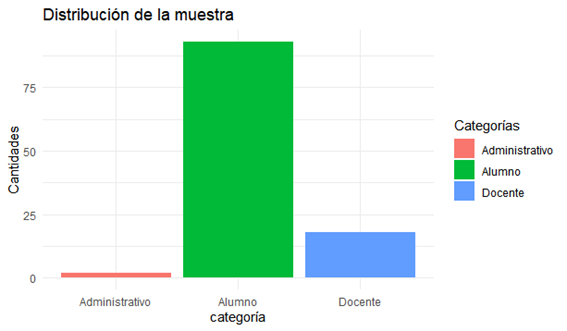
\includegraphics[width=0.5\textwidth]{Imagen2.png}
\caption{\label{fig:Imagen2}Distribución de la muestra.}
\end{figure}

La encuesta fue respondida por 113 personas, entre alumnos, docentes y administrativos. Realizamos el análisis de los datos usando R (En el Anexo I puede verse un ejemplo del código realizado en RStudio). En la fig. \ref{fig:Imagen2} puede observarse la distribución de la muestra.

La muestra tiene una mayoría de alumnos, así es que es posible que los resultados obtenidos tengan un “sesgo” por el rango etario de los alumnos.

A continuación, la encuesta preguntaba sobre el uso que hacen tanto docentes como alumnos y administrativos de los servicios en línea, utilizando una escala lineal, donde 1 implica que nunca hacen trámites en línea y 5, que siempre lo hacen. Los resultados, independientemente de la categoría, puede verse en la fig. \ref{fig:Imagen3}

\begin{figure}
\centering
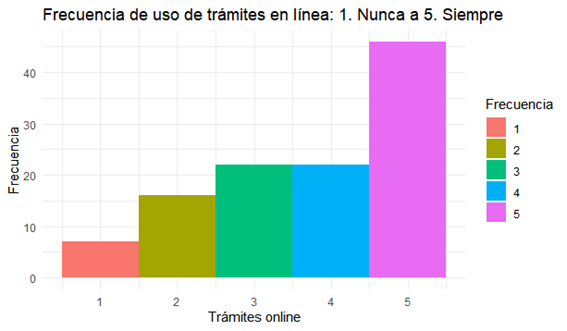
\includegraphics[width=0.5\textwidth]{Imagen3.png}
\caption{\label{fig:Imagen3}Uso de servicios en línea.}
\end{figure}

Como puede observarse, el histograma nos permite ver una distribución sesgada a la izquierda, con la mayoría de los valores agrupados en la opción 5, es decir, quienes realizan todos los trámites que pueden en línea. 

Sin embargo, hay un número de personas que aún no realizan todos los trámites en línea. Es por eso que, una de las cuestiones que involucra nuestro proyecto es la educación digital del ciudadano para el uso de estas tecnologías. 

Otra cuestión relacionada tiene que ver con la capacitación de los ciudadanos para el uso de estas tecnologías según el rango de edad (ver fig \ref{fig:Imagen4}. En el gráfico de barras puede observarse que, a medida que aumenta la edad, menor capacitación tienen los individuos. Esto tenderá a desaparecer naturalmente con el tiempo, cuando las generaciones sean todas nativos digitales, o se hayan adaptado a la digitalización.

\begin{figure}
\centering
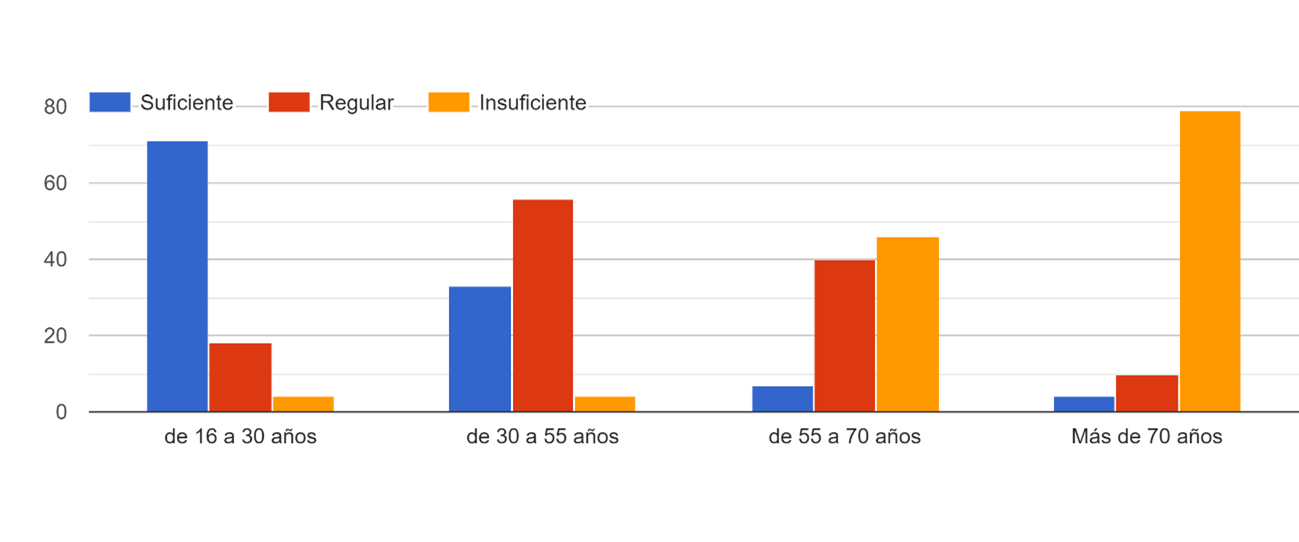
\includegraphics[width=0.5\textwidth]{Imagen4.png}
\caption{\label{fig:Imagen4}Capacitación digital de los ciudadanos según rango etario.}
\end{figure}

\subsubsection{Otros resultados}
\begin{figure}
\centering
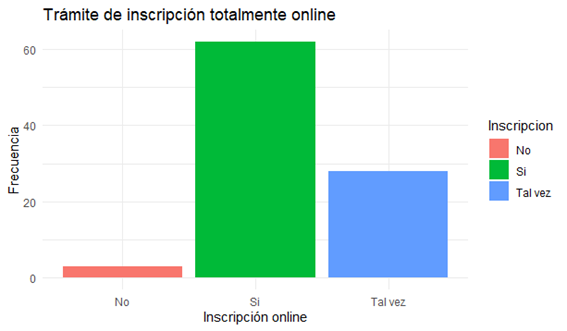
\includegraphics[width=0.5\textwidth]{Imagen5.png}
\caption{\label{fig:Imagen5}Trámite de inscripción en línea}
\end{figure}
\begin{figure}
\centering
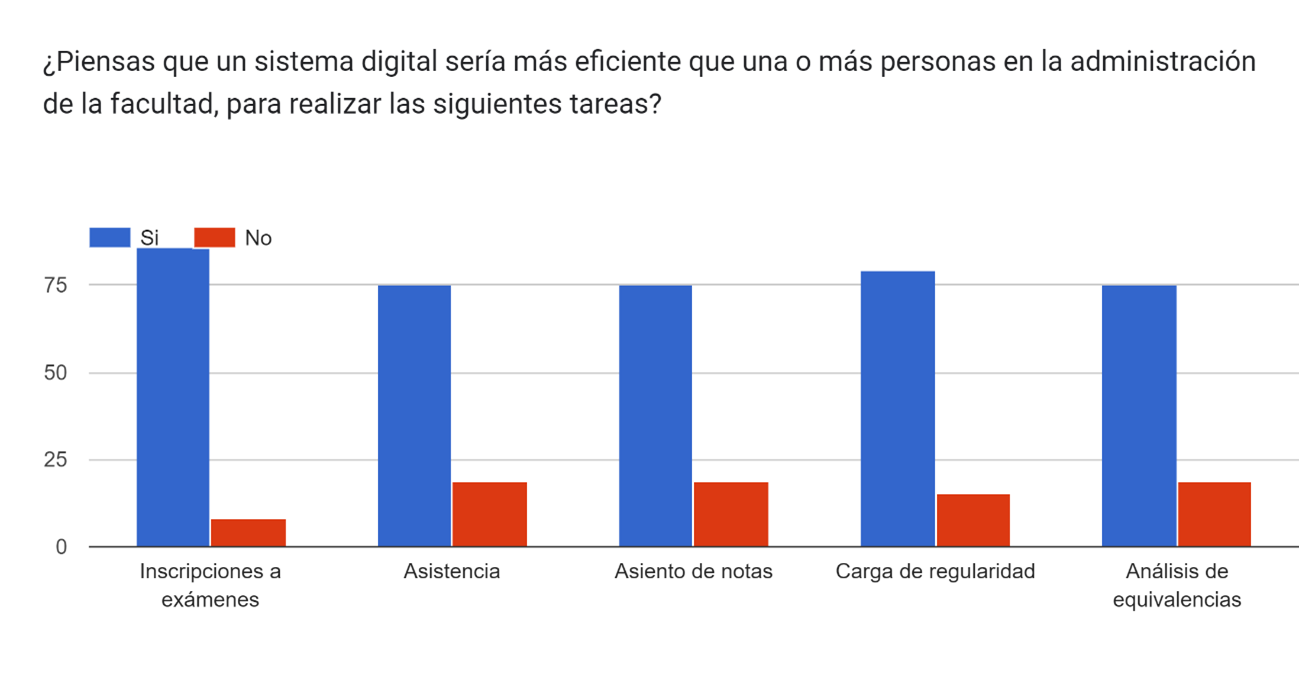
\includegraphics[width=0.5\textwidth]{Imagen6.png}
\caption{\label{fig:Imagen6}Eficiencia del sistema con otros trámites}
\end{figure}
\begin{figure}
\centering
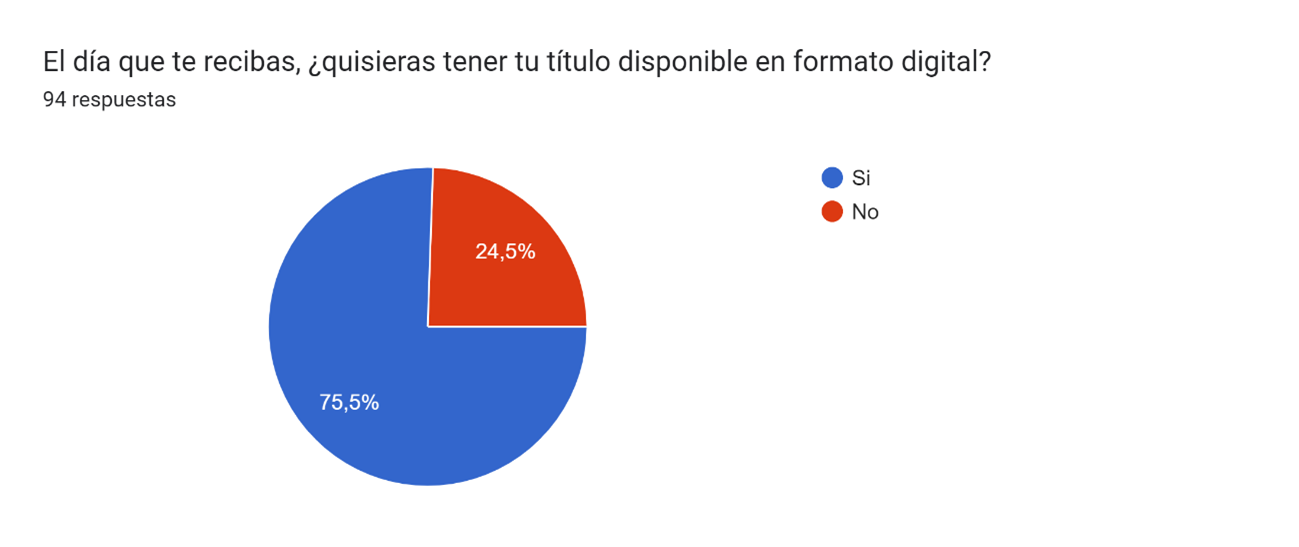
\includegraphics[width=0.5\textwidth]{Imagen7.png}
\caption{\label{fig:Imagen7}Títulos: ¿digitales o físicos?}
\end{figure}
Con respecto a los trámites a realizarse en la facultad, se plantean las siguientes preguntas:

¿El trámite de inscripción debería ser totalmente en línea? ver fig \ref{fig:Imagen5}. 

Las entrevistas informales nos permiten deducir que, los alumnos que superan el rango de los 35 años prefieren el formato presencial. Algunos estudiantes de menos de 20 años, aunque eligen el formato en línea, plantean también la necesidad de una atención presencial para recibir asesoramiento en persona. 
Algunas de las tareas que realiza la parte administrativa fueron incluidas en la encuesta para que los alumnos respondieran si les parece que las mismas serían más eficientes realizadas por sistema. Las respuestas pueden verse en la fig \ref{fig:Imagen6}. También se preguntó acerca de la posibilidad de tener el título en formato digital (fig \ref{fig:Imagen7}. 

En Mendoza, la Dirección General de Escuelas, ha adoptado un sistema donde se lleva el registro de la trayectoria académica de los alumnos. La fig \ref{fig:Imagen8} muestra que, quienes lo conocen, casi la mitad lo encuentra ineficiente. El sistema es relativamente nuevo, y ha ido mejorando año a año. Los docentes son, en general, quienes más se resisten, pero estimamos que esto es por la falta de capacitación en el uso de sistemas informáticos. 
Somos conscientes de que implementar un sistema lleva su tiempo de mejoras, aprendizajes, y necesita una red de conectividad que es posible que no contemos aún en nuestro país. Razón más para insistir en la inclusión de estas tecnologías para obligar a la modernización del sistema y a la capacitación de los usuarios. No se puede pensar en crecer como instituciones, como empresas, como regiones, si no contamos con estas herramientas. 

\begin{figure}
\centering
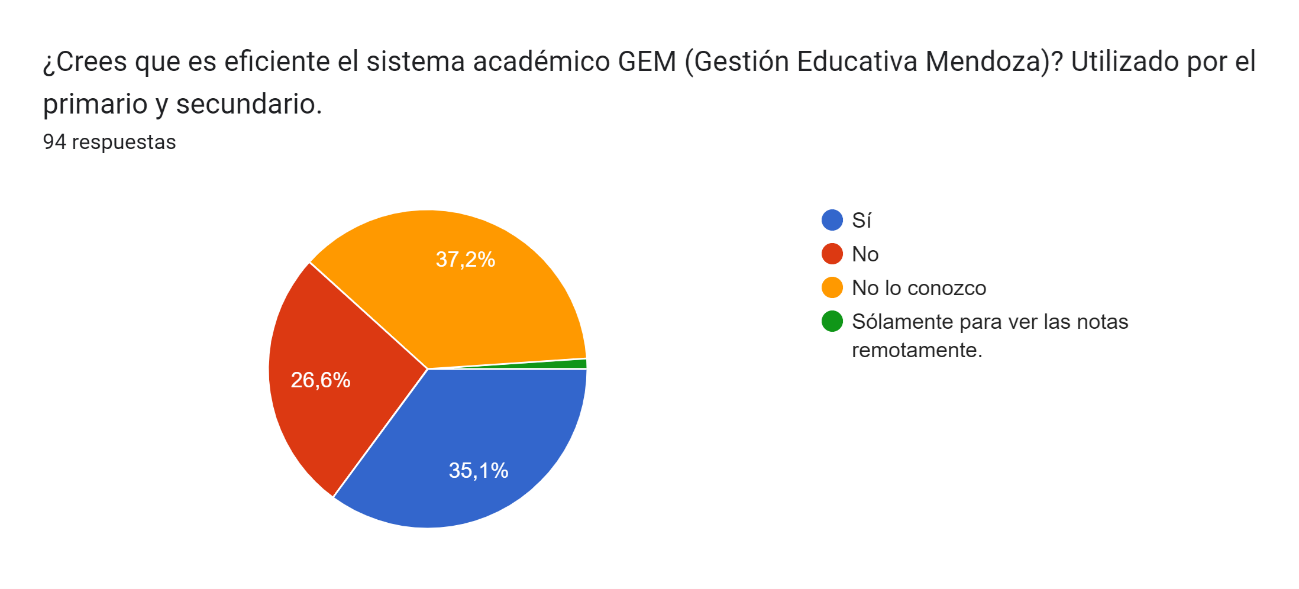
\includegraphics[width=0.5\textwidth]{Imagen8.png}
\caption{\label{fig:Imagen8}Eficiencia del sistema GEM.}
\end{figure}
\begin{figure}
\centering
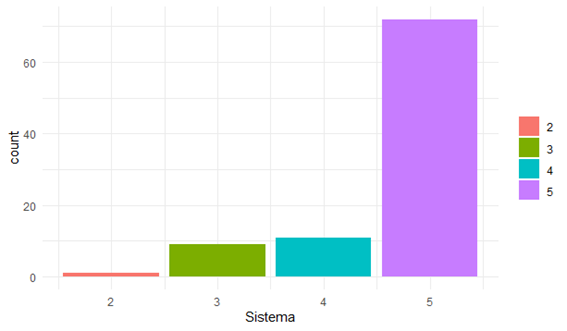
\includegraphics[width=0.5\textwidth]{Imagen9.png}
\caption{\label{fig:Imagen9}Solicitar y recibir documentación en línea.}
\end{figure}


Cuando se les pregunta a los alumnos qué tal útil le resultaría poder obtener toda la documentación necesaria (certificados, registros, actas, etc.) por sistema, en una escala lineal, de 1 a 5, donde 1 representa “nada útil” y 5 “muy útil”, observamos la distribución de frecuencias de la fig \ref{fig:Imagen9}.

\section{Análisis competitivo}

FODA son las siglas que representan al estudio de las Fortalezas, las Oportunidades, las Debilidades y las Amenazas de una empresa en un mercado. 
Realizamos la matriz FODA (ver fig \ref{fig:Imagen10} de nuestra propuesta teniendo en cuenta que el objetivo es automatizar procesos convirtiéndolos en más eficientes y sustentables, logrando disminuir el uso de recursos económicos, humanos y de tiempo.

\begin{figure}
\centering
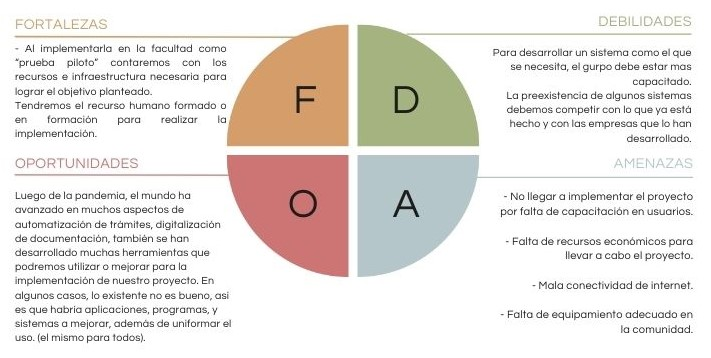
\includegraphics[width=0.5\textwidth]{Imagen10.jpg}
\caption{\label{fig:Imagen0}Matriz FODA.}
\end{figure}

% * <stephmigoni@gmail.com> 2018-02-08T19:23:33.559Z:
% 
% Esto es un comentario de prueba
% 
% 

%Puedes añadir comentarios en el ícono + del menú de arriba.

%Para responder a un comentario, simplemente da click en Reply en Rich Text.

%También pueden añadirse comentarios en el margen del pdf compilado con el comando todo \todo{¡Comment en el margen!}, como se muestra en el ejemplo de la derecha. También puedes añadirlos dentro del texto:

%\todo[inline, color=green!40]{Este es un comentario dentro del texto.}

%\subsection{¿Cómo añadir tablas en mi \TeX?}

%Usa los comandos table y tabular para iniciar una tabla simple --- mira la tabla~\ref{tab:tabla ejemplo}, como ejemplo. 

%\begin{table}
%\centering
%\begin{tabular}{l c r} 
%nùmero de columnas: 3
%l para left & c para centro & r para derecha \\ \hline
%Ejemplo & Centrado & Alineado a la\\
%Izquierda & 13 & Derecha
%\end{tabular}
%\caption{\label{tab:tabla ejemplo}Una simple tabla.}
%\end{table}

%\subsection{¿Cómo escribir (expresiones) Matemáticas?}

%\LaTeX{} es buenísimo para escribir ecuaciones. Para escribir variables o ecuaciones dentro del texto lo podemos poner entre signos de pesos y luego podemos seguir escribiendo, esto funciona si queremos escribir un símbolo como $\nabla$, $\pi$, $\beta$, $\Omega$, $\aleph$, etc.
%\begin{equation}
%\sum_{n=0}^\infty \frac{x^n}{n!}=e^x
%\end{equation}
%\begin{equation}


\subsection{Citas - falta}

%\bibliographystyle{abbrv}
%\bibliography{sample}

\end{document}